\documentclass[11pt]{article}
% =====================================================================
%  GRIM-pro (GRIM-P) family --- the two program-feature categories.
%  Companion to i2s_pro_categories.tex / i2s_anti_categories.tex.
%  Every cited branch + value is REAL (from bench/dataset.jsonl +
%  step5b_new_v3/grimoire_structural_WL/assignments_{s4,sB}.json + the
%  per-branch cards). Compile: pdflatex grim_pro_categories.tex
%  (needs tikz + pgfplots + listings + booktabs)
% =====================================================================
\usepackage[margin=1in]{geometry}
\usepackage{amsmath,amssymb}
\usepackage{xcolor}
\usepackage{listings}
\usepackage{booktabs}
\usepackage{tikz}
\usepackage{pgfplots}
\pgfplotsset{compat=1.16}
\usetikzlibrary{arrows.meta,positioning,shapes.geometric}

\definecolor{winc}{RGB}{30,120,60}   % winner (grimoire resolves) green
\definecolor{losc}{RGB}{190,60,60}   % loser  (cmplog / naive blocks) red
\definecolor{codebg}{RGB}{246,246,248}
\definecolor{kw}{RGB}{40,60,150}
\definecolor{cmt}{RGB}{120,120,120}
\definecolor{str}{RGB}{160,60,20}

\lstdefinestyle{c}{
  language=C, basicstyle=\ttfamily\small, backgroundcolor=\color{codebg},
  keywordstyle=\color{kw}\bfseries, commentstyle=\color{cmt}\itshape,
  stringstyle=\color{str}, numbers=none, frame=single, framerule=0pt,
  framesep=6pt, breaklines=true, showstringspaces=false, xleftmargin=4pt,
}

% tool / metric / rule / real-example box
\newcommand{\metricbox}[4]{%
  \par\smallskip\noindent\fbox{\parbox{\dimexpr\linewidth-2\fboxsep-2\fboxrule}{%
  \footnotesize
  \textbf{Tool:}~\texttt{#1}\\[2pt]
  \textbf{Metric:}~#2\\[2pt]
  \textbf{Verify rule (the arbiter fires this, no LLM):}~\texttt{#3}\\[2pt]
  \textbf{Real example:}~#4}}\par\smallskip}

\title{\textbf{The GRIM-pro family: two ways grammar-aware recombination gets through}}
\author{}
\date{}

\begin{document}
\maketitle
\vspace{-3em}

\paragraph{Backdrop.} \emph{GRIM-pro} (GRIM-P) collects the roadblocks where
\emph{grimoire} --- a structure-aware mutator that learns coherent input
fragments (its \texttt{GeneralizationStage} gaps-and-preserves whole runs) and
\emph{splices/recurses} them back together --- gets through, while a byte-level
fuzzer stays stuck. Where I2S-pro is ``the key was lying beside the lock''
(paste \emph{one} exact literal), GRIM-pro is ``assemble the whole grammatically
valid structure'': not one token, but a \emph{recombination of several coherent
constructs} into a larger, deeper input the parser/shaper will actually walk
into. Both categories below share that move; they differ only in whether the
advantage shows up as a \emph{countable richer set of structural tokens} or as
\emph{sheer size/depth} with no countable tag vocabulary. Counts are validated
roadblocks ($n$); the family total is $11$.

\smallskip\noindent\textit{Why the loser matters.} For most of these branches the
\emph{blocking} arm is \texttt{cmplog} (the decisive pair is
\mbox{grimoire\,$\succ$\,cmplog}), and that makes the test unusually sharp:
\texttt{cmplog}'s input-to-state \emph{can} paste an individual 4-byte table-tag
literal directly. So if the gate were cleared merely by \emph{placing a literal},
cmplog would match grimoire and the token advantage would vanish. A positive
token lift \emph{against the I2S arm} is what isolates grammar-aware
\emph{multi-token recombination} from plain literal substitution.

\smallskip\noindent\textit{A note on the metric.} All of GRIM-P is scored by one
registry tool, \texttt{joint\_necessity} in its generic two-arm
\texttt{analyze\_pair} mode, repointed to (\,winner $=$ \texttt{grimoire},
loser $=$ \texttt{cmplog} \emph{or} \texttt{naive}\,). It reports
\texttt{grimoire\_tags} (mean number of \emph{distinct} structural tokens per
grimoire seed), \texttt{tag\_lift} (that mean \emph{minus} the loser's), and
\texttt{size\_lift} (median seed-size \emph{ratio} grimoire/loser). The token
vocabulary is a per-target \emph{measurement parameter}, not a new tool: for
\texttt{harfbuzz} it is the 4-byte sfnt table tags ($+$ \texttt{ttcf}/\texttt{OTTO}
magic), for \texttt{libxml2} the XML/DTD constructs (\texttt{<?xml},
\texttt{<!DOCTYPE}, \texttt{xmlns}, \texttt{<!ELEMENT}, \texttt{/>}, \ldots).

% =====================================================================
\section*{1.\ \ Grimoire builds more structure \hfill {\normalsize\texttt{grimoire\_structural\_assembly} ($n=11$)}}
Grimoire's grammar-aware recombination clears the gate by assembling \emph{more
structure} than the byte/I2S loser. This surfaces through \textbf{two measurement
routes}: a countable \emph{token} lift (route~A --- richer distinct structural
tokens, surviving even against the I2S arm) or, where there is no tag vocabulary
to count, sheer recombined \emph{size/depth} (route~B). Same mechanism (grammar
recombination assembles structure), two handles; which fires is a property of the
gate. (We earlier split these as two categories --- \emph{structural\_token\_assembly}
($9$) and \emph{structural\_size\_depth} ($2$) --- but they are one mechanism with
two routes, merged 2026-06-26.)

\paragraph{Route A --- token assembly (\texttt{tag\_lift}).} The gate is cleared
only once the input carries \emph{several} coherent
structural constructs at once --- a font with multiple valid sfnt tables so the
shaper resolves a real script, or a nested XML document with namespace-bearing
attributes so the SAX path is actually walked. Grimoire builds these by splicing
learned fragments; the byte/I2S loser places few or none.

\begin{lstlisting}[style=c]
// harfbuzz  hb-ot-shaper.hh : hb_ot_shaper_categorize()
// dispatch needs planner->props.script to resolve to a real complex script
switch (script) {
  ...
  case HB_SCRIPT_GRANTHA:   // <-- blocker (harfbuzz/6181): needs a
                            //     structurally valid multi-table font
}
\end{lstlisting}

\noindent\textbf{How we know it is recombination, not a pasted literal.}
\texttt{cmplog} (the blocking arm here) \emph{can} splice a single 4-byte table
tag via I2S. If that were enough, its seeds would carry as many distinct sfnt
tokens as grimoire's and \texttt{tag\_lift} would collapse to $0$. Instead the
grimoire corpus carries \emph{several more} distinct tokens per seed, and is much
larger --- the signature of assembling a coherent multi-table structure rather
than dropping one literal.

\metricbox{joint\_necessity (analyze\_pair, winner=grimoire / loser=cmplog$|$naive)}
{\texttt{grimoire\_tags} (mean distinct structural tokens per seed), \texttt{tag\_lift} $=$ \texttt{grimoire\_tags} $-$ loser\_tags, \texttt{size\_lift} $=$ median size ratio grimoire/loser}
{tag\_lift >= 1.0 AND grimoire\_tags >= 2 AND size\_lift >= 1.0\ \ (cmplog route); \ tag\_lift >= 1.0 AND naive\_tags < grimoire\_tags AND grimoire\_tags >= 2\ \ (naive route)}
{harfbuzz/6181 (\texttt{hb\_ot\_shaper\_categorize}, \texttt{case HB\_SCRIPT\_GRANTHA}) --- vs the I2S arm: \texttt{grimoire\_tags}$=5.5$ but \texttt{cmplog\_tags}$=0.9$, so \texttt{tag\_lift}$=4.6$ with \texttt{size\_lift}$=7.83$. The seven \texttt{libxml2} branches (\texttt{6924/6925/6926/6948/6950/7147/7327}) take the \emph{naive} route, e.g.\ \texttt{6924} (\texttt{xmlNewNs}, nested-namespace path): \texttt{grimoire\_tags}$=6.1$ vs \texttt{naive\_tags}$=2$, \texttt{tag\_lift}$=4.1$.}

\begin{center}
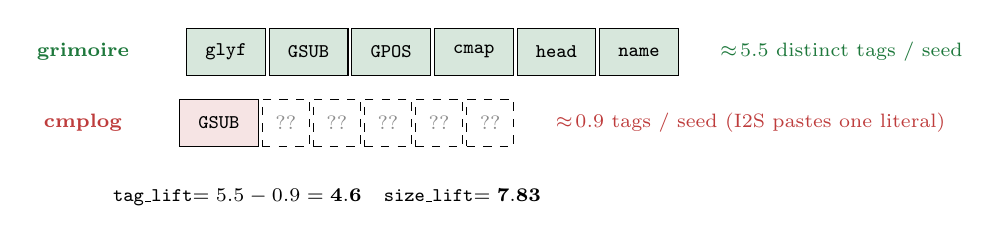
\begin{tikzpicture}[font=\footnotesize,
  tok/.style={draw,minimum height=6mm,minimum width=10mm,font=\scriptsize\ttfamily,inner sep=1pt},
  gap/.style={draw,dashed,minimum height=6mm,minimum width=6mm,font=\scriptsize,inner sep=1pt,text=black!45},
  lab/.style={font=\scriptsize\bfseries}]
% --- grimoire seed: many distinct coherent tokens ---
\node[lab,text=winc] (gl) at (0,0.9) {grimoire};
\node[tok,fill=winc!18,right=6mm of gl] (t1) {glyf};
\node[tok,fill=winc!18,right=1pt of t1] (t2) {GSUB};
\node[tok,fill=winc!18,right=1pt of t2] (t3) {GPOS};
\node[tok,fill=winc!18,right=1pt of t3] (t4) {cmap};
\node[tok,fill=winc!18,right=1pt of t4] (t5) {head};
\node[tok,fill=winc!18,right=1pt of t5] (t6) {name};
\node[right=4mm of t6,font=\scriptsize,text=winc] {$\approx\!5.5$ distinct tags / seed};
% --- cmplog seed: one literal + gaps ---
\node[lab,text=losc] (cl) at (0,0) {cmplog};
\node[tok,fill=losc!14,right=6mm of cl] (c1) {GSUB};
\node[gap,right=1pt of c1] (c2) {??};
\node[gap,right=1pt of c2] (c3) {??};
\node[gap,right=1pt of c3] (c4) {??};
\node[gap,right=1pt of c4] (c5) {??};
\node[gap,right=1pt of c5] (c6) {??};
\node[right=4mm of c6,font=\scriptsize,text=losc] {$\approx\!0.9$ tags / seed (I2S pastes one literal)};
% --- lift callout ---
\node[font=\scriptsize,align=center] at (3.1,-0.95)
  {\texttt{tag\_lift}$=5.5-0.9=\mathbf{4.6}$\quad\texttt{size\_lift}$=\mathbf{7.83}$};
\end{tikzpicture}\\[2pt]
{\footnotesize \texttt{harfbuzz/6181}: I2S can splice the \emph{one} \texttt{GSUB}
tag it logged, but it cannot \emph{recombine} a coherent multi-table font.
\texttt{joint\_necessity} counts the distinct structural tokens each corpus
carries; the gap between $5.5$ and $0.9$ is the grammar-recombination advantage
that survives even against an I2S arm.}
\end{center}

% =====================================================================
\paragraph{Route B --- size / depth (\texttt{size\_lift}).} The fallback handle.
The gate is about state-machine \emph{depth} or repeated
category structure rather than a countable target vocabulary, so the distinct-tag
count barely moves --- yet grimoire still wins because its recombined seeds are
materially \emph{larger and deeper}, driving the parser/shaper further into the
input. We consult this rule only when the token-assembly test above does
\emph{not} fire, and it keys on size alone.

\begin{lstlisting}[style=c]
// harfbuzz  hb-ot-shaper-thai.cc : get_consonant_type()
if (u == 0x0E0Eu || u == 0x0E0Fu)   // <-- blocker (harfbuzz/5958):
                                    //     needs a 0x0E0E/0x0E0F run inside a
                                    //     deep generalized glyph-buffer scaffold
\end{lstlisting}

\noindent The gate needs a specific Thai consonant codepoint reached only deep
inside a recombined glyph buffer. There is no table-tag vocabulary to count
(\texttt{tag\_lift}$\approx 0$); the discriminating signal is that grimoire's
seeds are several times larger than the loser's.

\metricbox{joint\_necessity (analyze\_pair, winner=grimoire / loser=cmplog)}
{\texttt{size\_lift} $=$ median grimoire seed size $/$ median loser seed size (consulted only when the token-assembly rule does not fire)}
{size\_lift >= 1.3}
{harfbuzz/5958 (\texttt{get\_consonant\_type:57}) --- \texttt{size\_lift}$=4.21$ (grimoire median $429.5$ B vs cmplog $102$ B) with \texttt{tag\_lift} only $0.7$. The other member, \texttt{libxml2/6743} (\texttt{xmlParseStartTag2}, attribute-defaulting path), has \texttt{size\_lift}$=2.22$ with \emph{no} positive tag lift ($-1.6$): pure depth, not token richness.}

\begin{center}
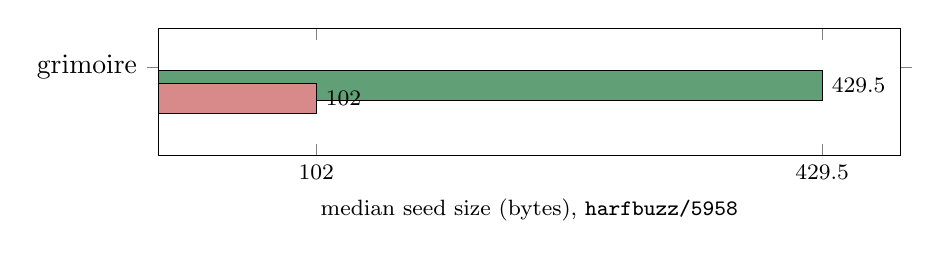
\begin{tikzpicture}
\begin{axis}[
  width=11cm, height=3.2cm, xbar, xmin=0, xmax=480,
  bar width=11pt, enlarge y limits=0.8,
  symbolic y coords={cmplog, grimoire},
  ytick=data, xtick={102,429.5}, xticklabel style={font=\footnotesize},
  nodes near coords, every node near coord/.append style={font=\footnotesize},
  xlabel={\footnotesize median seed size (bytes), \texttt{harfbuzz/5958}},
]
\addplot[fill=winc!70] coordinates {(429.5,grimoire)};
\addplot[fill=losc!60] coordinates {(102,cmplog)};
\end{axis}
\end{tikzpicture}\\[-2pt]
{\footnotesize When there is no tag vocabulary to count, sheer recombined
size/depth ($4.21\times$ here) is what carries grimoire past the gate.}
\end{center}

% =====================================================================
\section*{At a glance}
\begin{center}\small
\begin{tabular}{@{}p{3.8cm}clp{5.0cm}@{}}
\toprule
\textbf{Category} & \textbf{$n$} & \textbf{Example} & \textbf{One-line reason} \\
\midrule
structural assembly & 11 & harfbuzz/6181 (A), harfbuzz/5958 (B) & grammar recombination assembles more structure --- \textbf{route A} recombine several coherent tokens, surviving even the I2S arm (\texttt{tag\_lift}$\ge 1$); \textbf{route B} sheer recombined size/depth when no tag vocabulary (\texttt{size\_lift}$\ge 1.3$) \\
\midrule
\textbf{GRIM-P total} & \textbf{11} & & all scored by \texttt{joint\_necessity} analyze\_pair, winner $=$ grimoire \\
\bottomrule
\end{tabular}
\end{center}

\noindent\footnotesize All counts and metric values are from
\texttt{bench/dataset.jsonl} and
\texttt{step5b\_new\_v3/grimoire\_structural\_WL/assignments\_\{s4,sB\}.json};
the verify rules are the deterministic arbiter rules (no LLM in the decision).
The harfbuzz corpora live on server~\texttt{s4}, the libxml2 corpora on
server~\texttt{sB}; gates are quoted from the per-branch analysis cards.
\end{document}
